\section{译者补充:经典电磁理论下的光学基础}\label{sec:译者补充:经典电磁理论下的光学基础}
\begin{remark}
    本节内容不是原书内容,而是译者根据《Optics》\citep{hecht2016optics}
    补充并参考\citet{OpticsChinese}翻译的,请酌情参考和斧正。
    本节内容只简要介绍相关基础概念和结论,
    并不像正式的物理和光学教材那样严谨,请读者批判性地看待本节内容。
    本节要求读者具备较好的微积分与电磁理论知识储备。
    此外读者需注意,本节遵循有关内容惯例采用右手坐标系,
    与正文pbrt采用的左手坐标系不同。
\end{remark}

\subsection{波动}\label{sub:波动}
光的本质是什么?光是波动现象还是粒子现象?
这个问题非常复杂。早在二十世纪,物理学家们就已经发现,
光的电磁理论的经典结论在微观层级上完全不成立。
然而当我们站在通常的大尺度视角下,电磁波及其经典理论已经够用了。
为了打好基础,我们从波的数学描述说起,它也适用于一切物理波。

\subsubsection*{一维波}
行进中的\keyindex{波}{wave}{}的一个本质特性是,
它是传播波的\keyindex{介质}{medium}{}的自持\keyindex{扰动}{disturbance}{}。
\keyindex{机械波}{mechanical wave}{wave\ 波}是
我们最熟悉的波,例如琴弦上的波、液体表面的波以及
空气中的\keyindex{声波}{sound wave}{wave\ 波}。
\begin{definition}[\keyindex{纵波}{longitudinal wave}{wave\ 波}]
    介质在波动方向上位移。
\end{definition}
\begin{definition}[\keyindex{横波}{transverse wave}{wave\ 波}]
    介质位移的方向垂直于波动方向。
\end{definition}
\begin{example}
    声波是纵波;琴弦上的波、电磁波是横波。
\end{example}
波区别于粒子流的几个关键特征之一是,
扰动在前进,但实物介质并不前进。
就像风吹起滚滚麦浪,但麦穗只是原地摇摆。
\begin{figure}[htbp]
    \centering
    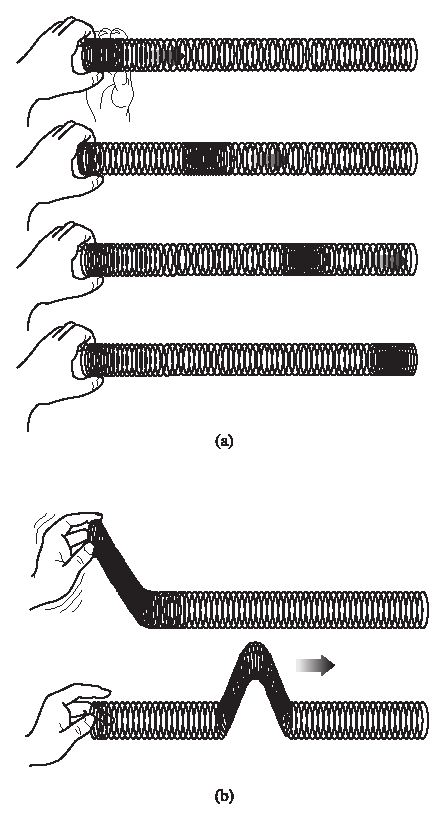
\includegraphics[width=0.65\linewidth]{Pictures/chap08/longitudinalAndTransverseWave.eps}
    \caption{弹簧中的(a)纵波;(b)横波。}
    \label{fig:08ex02.0201}
\end{figure}

我们暂不追究扰动的本质,而专注研究描述波动的方程应该具备怎样的形式。
设某个这样的扰动$\psi$以恒定速度$v$沿正$x$方向运动。
既然扰动在运动,则它必然是位置和时间的函数:
\begin{align}
    \psi(x,t)=f(x,t)\, ,
\end{align}
其中$f(x,t)$对应于某个具体函数或波形。
如\reffig{08ex02.0203}(a)所示,一个脉冲在静止坐标系$S$中以速度$v$运动。
我们取定任意时刻$t$即可得到那个时刻波的\keyindex{剖面}{profile}{},
就像脉冲经过时给它“拍照”。例如$t=0$有
\begin{align}
    \psi(x,t)\bigg|_{t=0}=f(x,0)=f(x)
\end{align}
表示0时刻波的剖面。
\begin{figure}[htbp]
    \centering
    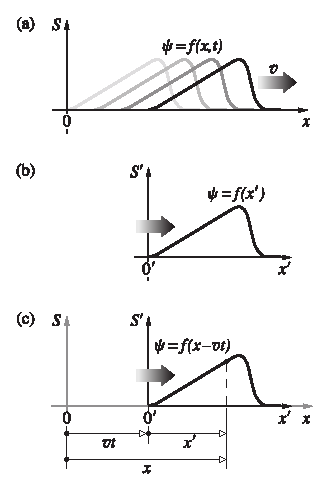
\includegraphics[width=0.5\linewidth]{Pictures/chap08/MovingReferenceFrame.eps}
    \caption{运动参考系。}
    \label{fig:08ex02.0203}
\end{figure}

现在,我们先只考虑传播时形状不变的波。
在一段时间$t$后,脉冲沿$x$轴前进了距离$vt$,其余不变。
如\reffig{08ex02.0203}(b),我们引入新坐标系$S'$并与脉冲以相同速度$v$运动。
则在该坐标系中$\psi$不再是时间的函数,而是静止不变的剖面,即
\begin{align}
    \psi=f(x')\, ,
\end{align}
这意味着坐标系$S'$中的扰动在任意时刻$t$的形状,
都和$S$中$t=0$时两者具有同一原点时扰动的形状相同,如\reffig{08ex02.0203}(c)所示。
为了将上式改写为$S$中某静止观察者描述的形式,我们利用
\begin{align}
    x'=x-vt
\end{align}
得到
\begin{align}
    \psi(x,t)=f(x-vt)\, .
\end{align}
上式是一维\keyindex{波函数}{wave function}{wave\ 波}的最一般形式。
它描述了一个具有所需剖面形状$f(x)$的波,它以速度$v>0$沿正$x$方向运动。
相似地,如果波向负$x$方向运动,则上式应改写为
\begin{align}
    \psi(x,t)=f(x+vt)\, .
\end{align}
总之变量$x$和$t$一定作为一个整体变量$x\mp vt$出现。

\subsubsection*{波动微分方程}
接下来我们推导一维波动方程的形式,把$\psi(x,t)$对空间与时间的依赖关系联系起来。注意到
\begin{align}
    \frac{\partial x'}{\partial x}=\frac{\partial (x\mp vt)}{\partial x}=1\, ,
\end{align}
以及
\begin{align}
    \frac{\partial x'}{\partial t}=\mp v\, ,
\end{align}
所以$\psi(x,t)$在$t$恒定时对$x$的偏微分为
\begin{align}
    \frac{\partial \psi}{\partial x}
    =\frac{\partial f}{\partial x}
    =\frac{\partial f}{\partial x'}\frac{\partial x'}{\partial x}
    =\frac{\partial f}{\partial x'}\, .
\end{align}
而在$x$恒定时$\psi(x,t)$对$t$的偏微分为
\begin{align}
    \frac{\partial \psi}{\partial t}
    =\frac{\partial f}{\partial t}
    =\frac{\partial f}{\partial x'}\frac{\partial x'}{\partial t}
    =\mp v\frac{\partial f}{\partial x'}
    =\mp v\frac{\partial \psi}{\partial x}\, .
\end{align}
上式表明$\psi$对$x$和$t$的变化率只差一个常系数。
继续求$\psi$的二阶偏微分有
\begin{align}
    \frac{\partial^2 \psi}{\partial x^2}
    =\frac{\partial}{\partial x}\left(\frac{\partial \psi}{\partial x}\right)
    =\frac{\partial}{\partial x}\left(\frac{\partial f}{\partial x'}\right)
    =\frac{\partial}{\partial x'}\left(\frac{\partial f}{\partial x'}\right)\frac{\partial x'}{\partial x}
    =\frac{\partial^2 f}{\partial x'^2}\, ,
\end{align}
并进一步得到
\begin{align}
    \frac{\partial^2 \psi}{\partial t^2}
    = & \frac{\partial}{\partial t}\left(\frac{\partial \psi}{\partial t}\right)
    =\frac{\partial}{\partial t}\left(\mp v\frac{\partial f}{\partial x'}\right)\nonumber    \\
    = & \mp v\frac{\partial}{\partial x'}\left(\frac{\partial f}{\partial t}\right)
    =\mp v\frac{\partial}{\partial x'}\left(\frac{\partial \psi}{\partial t}\right)\nonumber \\
    = & \mp v\frac{\partial}{\partial x'}\left(\mp v\frac{\partial f}{\partial x'}\right)
    =v^2\frac{\partial^2 f}{\partial x'^2}\nonumber                                          \\
    = & v^2\frac{\partial^2 \psi}{\partial x^2}\, .
\end{align}
整理上式即
\begin{definition}[一维\keyindex{波动微分方程}{differential wave equation}{equation\ 方程}]
    \begin{align}
        \frac{\partial^2 \psi}{\partial x^2}=\frac{1}{v^2}\frac{\partial^2 \psi}{\partial t^2}\, .
    \end{align}
\end{definition}
注意上式是一个\keyindex{齐次微分方程}{homogeneous differential equation}{equation\ 方程},
没有仅含独立变量的项(例如一份“力”或“源”),
所以描述的是\keyindex{无阻尼系统}{undamped system}{system\ 系统}。
这意味着若$\psi$是方程的解,则它乘以任意倍数后也是解。
反之,若一个波函数是上述方程的解,则它将是$x\mp vt$的函数,
且可以对$x$和$t$求得非平凡的二阶微分。

\subsubsection*{谐波}
最简单的波形是正弦或余弦曲线。它可以称作
\keyindex{正弦波}{sinusoidal wave}{wave\ 波}、
\keyindex{简谐波}{simple harmonic wave}{wave\ 波}
或\keyindex{谐波}{harmonic wave}{wave\ 波}。
任何波形都可以由谐波叠加合成。

我们为谐波波形选定为以下简单函数:
\begin{align}
    \psi(x,t)\bigg|_{t=0}=\psi(x)=f(x)=A\sin kx\, ,
\end{align}
其中常数$k>0$称作\keyindex{传播数}{propagation number}{},
$kx$这个整体是无量纲的。$\psi(x)$的最大值$A>0$称作波的\keyindex{振幅}{amplitude}{}。
将上式中的$x$替换为$x-vt$,改写成以速度$v$沿正$x$方向前进的波:
\begin{align}
    \psi(x,t)=A\sin k(x-vt) = f(x-vt)\, .
\end{align}
显然它是波动微分方程的一个解。该波在空间和时间中都具有周期性。
它的\keyindex{空间周期}{spatial period}{period\ 周期}
称作\keyindex{波长}{wavelength}{},表示每个波的长度,记作$\lambda$.
当$x$大小增减$\lambda$,$\psi$应不变:
\begin{align}
    \psi(x,t)=\psi(x\pm\lambda,t)\, .
\end{align}
这对应了正弦函数自变量改变$\pm2\pi$,由于$k>0,\ \lambda>0$,所以
\begin{align}
    k=\frac{2\pi}{\lambda}\, .
\end{align}
此外,正弦函数的自变量也称作\keyindex{相位}{phase}{},记作$\varphi$,
即有$\psi(x)=A\sin\varphi$.

类似得,$\psi$的\keyindex{时间周期}{temporal period}{period\ 周期}记作$\tau$,
可简称\keyindex{周期}{period}{},即一个完整的波经过一静止观察者的时间。
它对应了波在时间上的重复行为:
\begin{align}
    \psi(x,t)=\psi(x,t\pm\tau)\, .
\end{align}
由此我们容易推出
\begin{align}
    kv\tau=2\pi\, ,
\end{align}
以及
\begin{align}
    \tau=\frac{\lambda}{v}\, .
\end{align}

周期的倒数称作\keyindex{时间频率}{temporal frequency}{frequency\ 频率},
可简称\keyindex{频率}{frequency}{},记作$\nu$,即单位时间里波的个数
\sidenote{注意$\nu$是希腊字母。}:
\begin{align}
    \nu\equiv\frac{1}{\tau}\, ,
\end{align}
其单位为\keyindex{赫兹}{Hertz}{}(简写为Hz),即每秒周数。
结合前述定义,不难发现\keyindex{波速}{speed}{}$v$满足
\begin{align}
    v=\nu\lambda\, .
\end{align}

此外我们还定义\keyindex{时间角频率}{angular temporal frequency}{frequency\ 频率}为
\begin{align}
    \omega\equiv\frac{2\pi}{\tau}=2\pi\nu\, ,
\end{align}
可简称为角频率,单位为弧度每秒(rad/s)。

此外,\keyindex{空间频率}{spatial frequency}{frequency\ 频率},
也称\keyindex{波数}{wavenumber}{},定义为
\begin{align}
    \kappa\equiv\frac{1}{\lambda}\, ,
\end{align}
即单位长度中波的数目,单位为$\mathrm{m}^{-1}$.

以上所有概念也适用于非谐波,只要它是单个剖面元规则重复构成的。
